\documentclass{article}
\usepackage{graphicx} % new way of doing eps files
\usepackage{listings} % nice code layout
\usepackage[usenames]{color} % color
\usepackage{float}
\definecolor{listinggray}{gray}{0.9}
\definecolor{graphgray}{gray}{0.7}
\definecolor{ans}{rgb}{1,0,0}
\definecolor{blue}{rgb}{0,0,1}
% \Verilog{title}{label}{file}
\newcommand{\Verilog}[3]{
  \lstset{language=Verilog}
  \lstset{backgroundcolor=\color{listinggray},rulecolor=\color{blue}}
  \lstset{linewidth=\textwidth}
  \lstset{commentstyle=\textit, stringstyle=\upshape,showspaces=false}
  \lstset{frame=tb}
  \lstinputlisting[caption={#1},label={#2}]{#3}
}


\author{Jiasen Zhou and Jon Johnston}
\title{Lab 13}

\begin{document}
\maketitle

\section{Executive Summary}
The goal of the lab is adding the register buffers between each stage and get a simple pipeline working and then implement the 10 instruction (NOP doesn't count in). In this lab, the iFetch, iDecode, iExecute, Memory and Writeak stages are all connected together. the pipeline buffers are added between each stage based on the buffer table.NOP instruction are added because there is no dataforwarding and hazard detection. The lab was successful.


\section{Test Report}
To verify operation of the pipeline, this lab requires 1 test bench.
\begin{enumerate}
	\item Pipeline simulation
\end{enumerate}
\subsection{Pipeline Test Bench}
The Pipeline Test Bench contains:
\begin{enumerate}
	\item Inputs
	\begin{enumerate}
		\item branch\_target - branch address
		\item pc\_src - the control of branch mux
		\item reset - set the current pc to be 0
		
	\end{enumerate}	
	\item Outputs
	\begin{enumerate}	
		\item  control signals that stored in buffer 
	\end{enumerate}	
\end{enumerate} 
\pagebreak

\begin{figure}[H]
		\begin{center}
		\caption{Piepline buffer table.}\label{fig:ert_registertest}
		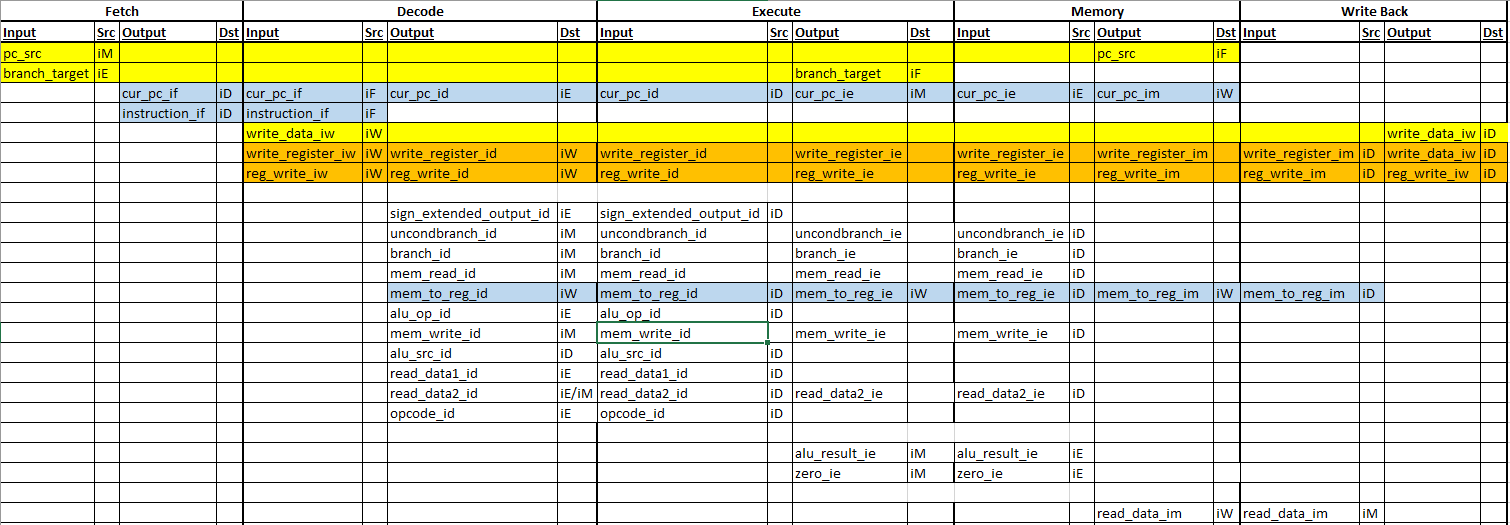
\includegraphics[width=1.0\textwidth]{../images/Lab12_pipelined_datapath_table.png}
	\end{center}
\end{figure}
\begin{figure}[H]
	\begin{center}
		\caption{Expected Results of the pipeline test.}\label{fig:ert_registertest}
		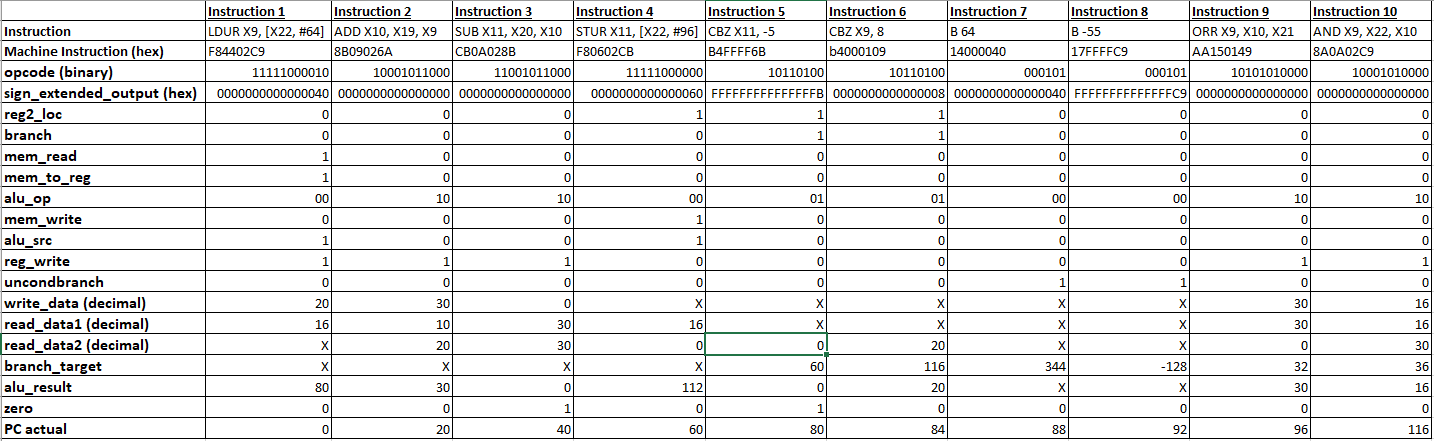
\includegraphics[width=1.0\textwidth]{../images/Lab13_pipeline_table.png}
	\end{center}
\end{figure}

\begin{figure}[H]
	\begin{center}
		\caption{Timing diagram for the pipeline test.}\label{fig:registertest}
		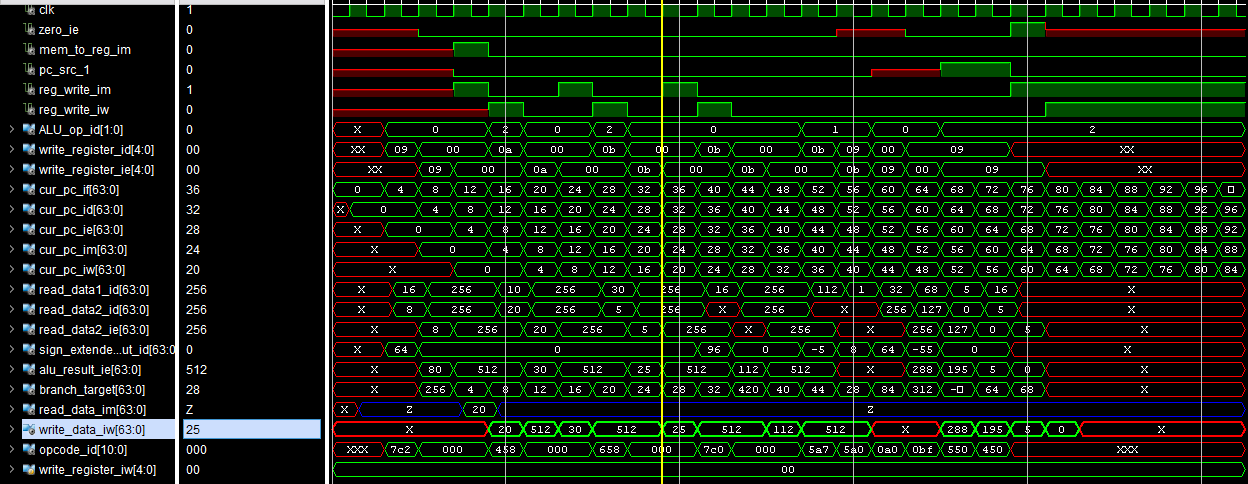
\includegraphics[width=1.0\textwidth]{../images/Lab13_pipeline_timing_diagram.png}
	\end{center}
\end{figure}


\section{Code Appendix}
% The code appendix should include the test bench code and module code for this lab.
\Verilog{Verilog code of piepline.}{code:regtest}{../code/2_decode/pipeline_datapath.v}

\end{document} 